\documentclass[a4paper]{article}
\usepackage[T1]{fontenc}
\usepackage{lmodern}
\usepackage{amssymb,amsmath}
\usepackage{ifxetex,ifluatex}
\usepackage{fixltx2e} % provides \textsubscript
% use microtype if available
\IfFileExists{microtype.sty}{\usepackage{microtype}}{}
\ifnum 0\ifxetex 1\fi\ifluatex 1\fi=0 % if pdftex
  \usepackage[utf8]{inputenc}
\else % if luatex or xelatex
  \usepackage{fontspec}
  \ifxetex
    \usepackage{xltxtra,xunicode}
  \fi
  \defaultfontfeatures{Mapping=tex-text,Scale=MatchLowercase}
  \newcommand{\euro}{€}
\fi
\ifxetex
  \usepackage[setpagesize=false, % page size defined by xetex
              unicode=false, % unicode breaks when used with xetex
              xetex]{hyperref}
\else
  \usepackage[unicode=true]{hyperref}
\fi
\hypersetup{breaklinks=true,
            bookmarks=true,
            pdfauthor={},
            pdftitle={MasterThesis/Thesis Proposal},
            colorlinks=true,
            urlcolor=blue,
            linkcolor=magenta,
            pdfborder={0 0 0}}
\setlength{\parindent}{0pt}
\setlength{\parskip}{6pt plus 2pt minus 1pt}
\setlength{\emergencystretch}{3em}  % prevent overfull lines
%\setcounter{secnumdepth}{0}

\title{Speeding up the performance of Parallel and Distributed Simulations using Haskell and laziness}
\author{Nikolaos Bezirgiannis}
\date{February 25, 2013}

\begin{document}

\begin{titlepage}
  \begin{center}

    {\LARGE Speeding up the performance of Parallel and Distributed Simulations
    using Haskell and laziness}\\[0.5cm]

    {\Large By}\\
    {\Large Nikolaos Bezirgiannis}\\[1.5cm]

    % Supervisor
    \begin{minipage}{0.8\linewidth}
      \begin{center}
    \begin{minipage}{0.4\textwidth}
      \begin{flushleft} \large
        \emph{Supervisor}\\
        Wishnu Prasetya
      \end{flushleft}
    \end{minipage}
    % Supervisor
    \begin{minipage}{0.5\textwidth}
      \begin{flushright} \large
        \emph{Supervisor}\\
        Johan Jeuring
      \end{flushright}
    \end{minipage}
    \end{center}
    \end{minipage}

    \vspace{1.5cm}

    {\Large MSc Thesis Proposal}

  \vfill
  
  
\includegraphics{uu_logo}

  {\large Dept. of Information and Computing Sciences,}\\
  {\large Utrecht University}\\[1cm]

  {\large February 25, 2013}

  \end{center}


\end{titlepage}

%% \begin{abstract}

%% \end{abstract}
%% 
\section{Introduction to Simulation}

Complex system (complex comes from Latin com-  together + plectere  to twine or braid) is a system composed from relatively many mutually related  parts.

As Greek philosopher Aristotle famously said, ``The whole is more than the sum of its parts''.
That means that there are emergent behaviours of a system that cannot be observed
when examining its pieces individually.

\subsection{Types of complex systems}

\begin{description}
\item[Structurally complex] \hfill \\
A complex system that has relatively few components, but many relations
between the components (E.g. airport traffic).
\item[Dynamically complex] \hfill \\
A complex system with extremely many components, that interact in trivial manner.
The behaviour of the system is emerging from these numerous interactions (E.g. virus contamination).
\end{description}

\subsection{Examples of complex systems\cite{burian_complex_????}}

Parts of human society:

\begin{itemize}
\item    Markets
\item    Organizations
\item    Language
\item    Internet
\end{itemize}

Biology:	
\begin{itemize}
\item    Cells
\item    Organ – e.g. brain
\item    Immune system
\item    Organisms
\item    Populations
\item    Ecosystem
\end{itemize}
	
Physics:

\begin{itemize}
\item    Turbulence
\item    Weather
\item    Percolation
\item    Sandpile
\end{itemize}


Complex systems are usually (but not always) intricated - hard to describe or understand\cite{burian_complex_????}. For this reason, we turn to simulation. 
Simulation is the imitation of the operation of a real-world process or system over time.
This allows us to reduce a complex system to a mere abstract model of it, that could be better
analyzed. A model is the algorithms and/or equations that best describe the behaviour of the system.

What we really do in simulation is estimating the real performance of a system, 
which is too complex to have an analytical solution. In that context,
simulation is applied to give answers to specific questions, i.e. decision support (E.g. how fast
is the system? , what is its bottleneck?, how can we maximize its throughput?)

\subsection{Applications of Simulation}

\subsubsection{Transportation}

Consider an unexpected hurricane affecting the air traffic of a country. 
How decision support is influenced? Should airplanes
be allowed to depart, only to circle on the destination?
Should airplanes be stay foot? Should there be some kind of rerouting
to alternative destinations? How much will be the frustration of the passengers (average waiting time)?

\subsubsection{Economics and Social Science}

Examples of these include, the effects of a surprising announcement on the stock market,
how a declaration of war will affect the economy, what is the better suited
economic model for the eurozone. A famous example of application in the Social Science,
is how the ghetto communities are formed even with high tolerance between the factions.

\subsubsection{Biology}

A possible spread of a virus is very catastrophic. Simulations can investigate
cases of virus contamination in the population, how the spreading works,
what are the best quarantine systems.

\subsubsection{Computer Systems}

An example could be the designing of a next-generation internet protocol.
How many web surfers are expected? How much will be the tolerance of delay? What
will happen in unexpected failures of the network?

\subsubsection{Weather Forecast}

Simulation models with a huge size are created and executed, to make future predictions 
about the weather in a country or even the change in the world climate.


\subsubsection{Military}

In wargaming, different military tactics and strategies are evaluated, so
as to determine the gear that is required. Simulation
can be also used as a training facility for the military personnel.


A simulation can be either calculated on pen-and-paper or executed automatically
using a computer. For the rest of this proposal we are only considering computer simulation.

\subsection{Discrete-event Simulation (DES)}

Every kind of computer simulation has to 
provide  (l) a representation of the state of the system, (2) some means of
changing this representation to model the evolution of the system, and (3)
some representation of time \cite{fujimoto_parallel_2001}.

In Discrete-event Simulation, as the name suggests we (1) represent
state with state variables, (2) change the state by occurring events,
(3) the time is discrete --- discontinuous jumps from event happening at time $t$ to next event's
time $t'$.


\subsection{Parallel and Distributed DES (PDES)}

Parallel and Distributed Simulation (PDES) refers to the execution
of a simulation on a computer system comprised of multiple machines,
interconnected through a network.

A definitive aspect of PDES is \emph{local causality constraint}: Events with the same timestamp are processed in the same order both in the sequential and parallel execution

Local causality constraint has the effect of:

\begin{itemize}
\item  Parallel/distributed execution yields the same results as sequential execution
\item The results of the simulation are reproducible
\end{itemize}


There are four advantages that PDES offers:

\begin{description}
\item[Faster execution] \hfill \\
It is the common case that users consider PDES when there are computational limitation on
executing the simulation on a single machine.
\item[Geographical distribution] \hfill \\
Users at different geographical places can participate on a simulation run, and
interact with other participants (called human-in-the-loop). An example
of this can be military training (war-gaming).
\item[Simulators of different machines] \hfill \\
PDES allows the connection and interaction of already-made simulation systems, such
that to create a larger simulation environment.
\item[Fault tolerance] \hfill \\
If a particular processor fails, another processor of the simulation system can pick up
its work, thus offering resistance to failure.
\end{description}

In both conservative and optimistic synchronization, the state is split
into pieces with each piece distributed to a logical process (LP) for computing it.
This is alternatively called \emph{space-parallel simulation}, in contrast
to \emph{time-parallel simulation}, describe later.
There is speedup observed, because the state is computed in parallel, compared
to a single execution of the state. This can be better depicted in a ``time-state'' graph.

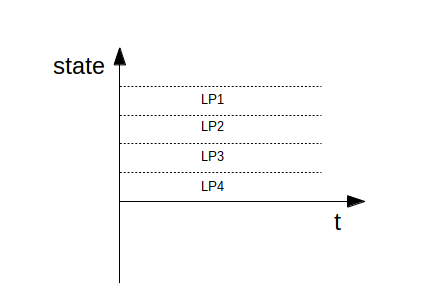
\includegraphics{thesis-proposal-space-graph}

\subsubsection{Conservative synchronization}

It's a synchronization mechanism, that guarantees that only \emph{safe events}
are processed by the Logical Process. An event is considered safe, if after its
processing there will be no prior events available for execution. For example,
an event $e$ with time $t$ is processed by the LP. If later, another
event $e'$ comes with time $t' < t$, then the event $e$ should not be processed
earlier than $e'$. The event $e$ was unsafe.

A critical term in conservative synchronization is lookahead. Lookahead
is a value measured in time, that allows an LP to safely process events.
For example, if there are 2 logical processes in the simulation, and $LP_1$ and
$LP_2$ and the lookahead is $l_{2-1} = 3$ then $LP_1$ knows that it
is safe to process events with time $e_i + l_2{-1} => e_i + 3$. Lookahead
between 2 logical processes $LP_j$ and $LP_i$ guarantees that an event triggered
at time $t_J$ in $LP_j$ will take at least $l_{ji}$ time steps to arrive/be scheduled
in $LP_i$. So $LP_i$ knows which events are safe to process. Alternatively,
lookahead can be considered as the ``distance'' between 2 logical processes.

There are many different algorithms to achieve this, the most famous being the
Chandy/Misra/Bryant null message protocol algorithm \cite{misra_distributed_1986}.

\subsubsection{Optimistic synchronization (Time Warp)}

In optimistic synchronization mechanism, an event could be processed unsafely, that
means that the timestamp order of events is violated. When this happens at an $LP_i$, the LP
has to rollback the state to the previous safe point, and replay the correct sequence
of events.

This is implemented with intermediate state saving; after each event is processed,
its generated state is saved to memory, only to be recalled if an unsafe event occurs.
Because the number states are ever increasing, so does memory. For this reason,
many fossil collection algorithms have been devised.

\subsubsection{Time-parallel simulation}

In time-parallel simulation, we split the time into time slices, and
distribute each to a logical process to compute individually. Although
there are big performance gains, not many discrete-event simulations are suited for
time-parallel simulation. For this reason, we do not take it into account in our proposal.
The ``time-state'' graph is illustrated as:

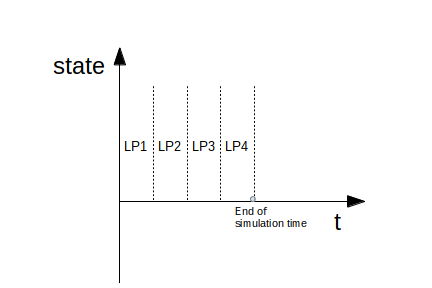
\includegraphics{thesis-proposal-time-graph}

\subsubsection{Related to PDES but not considered PDES technology}

\begin{description}
\item[Parameter Sweeping] \hfill \\
It is the process of varying parameter values and/or
random seeds of a model in an automated fashion, 
and distributing the different simulation instances in multiple machines for execution.
Parameter sweeping for NetLogo is described in \cite{koehler_clustered_2005}.
An example of a general-purpose parameter sweeping simulation system is \href{http://drone.sourceforge.net/}{Drone}.
\item[Load Balancing] \hfill \\
Multiple instances of a specific simulation model can be generated using parameter sweeping.
These instances are then distributed to multiple machines. It can be the case,
that during the execution, the workload of each machine is not evenly distributed.
Load balancing is required to guarantee a fair distribution of the workload and is
applied dynamically, during the execution of the simulation instances.
In ABM, load balancing can be realized through agent migration. Load balancing can also
be defined such that, it minimizes the intercommunication, which is the major bottleneck
in distributed systems. Further information can be retrieved from \cite{chow_load_2002}.

\item[Region Clustering] \hfill \\

It is only applied for grid-based models, i.e. models where entities have a single spatial
representation on a plane. It is similar to load balancing, albeit statically defined.

\end{description}



\section{Thesis Statement}

\subsection{Research Question}

How can we speed up the execution of Parallel and Distributed Discrete
Event Simulations (PDES) that have optimistic synchronization?

\subsection{Hypothesis}

A simulation event is associated with specific code that gets executed by the event handler.
This code is nothing more than state variable assignment statements.
E.g.

$$statevariable_1 = 0$$
$$statevariable_2 = statevariable_1 / 3$$
$$statevariable_3 = statevariable_1 + statevariable_2$$

Usually, the event code is executed with eager evaluation. This means
that state variables are evaluated down to normal form.

We hypothesize that we can execute associated simulation code using lazy evaluation only.
State variables are processed down to weak head normal form (WHNF).
This has 2 effects:

\begin{enumerate}
\item We can now express lazy programs in simulation environments. E.g. of a block event code:
\begin{equation}statevariable_1 = [1..]\end{equation}
\begin{equation}statevariable_2 = take \; 4 \; statevariable_1\end{equation}
\begin{equation}statevariable_3 = take \; 1 \; statevariabel_2\end{equation}

\item Code that is not needed in later events will not be executed. This means
that if code does not depend on previous code, then the previous code need not
to be executed. This intrinsic effect is the result of laziness. Consider
that after the above event block code, a new event block code comes that looks like this:

\begin{equation}statevariable_1 = [0..]\end{equation}
\begin{equation}statevariable_2 = 0\end{equation}
\begin{equation}statevariable_3 = 1\end{equation}

Then it would be a waste to fully compute the 
$statevariable_2 = take \; 4 \; statevariable_1$
and
$statevariable_3 = take \; 1 \; statevariabel_2$
in (2) and (3).

The end-result is that we are freeing the simulation-user from
being careful of what gets computed inside the simulation code.

\end{enumerate}


\subsection{Optional considerations}

\begin{description}
\item[Distributing simulation with Cloud Haskell] \hfill \\
Cloud Haskell is a distributed computing framework for Haskell. It
follows the Erlang philosophy to distribute work to multiple machines
over a network. We could make use of Cloud Haskell to distribute simulation
across many logical processes. A possible hint to consider is how
this affects the simulation laziness proposed.
\item[Parameter Sweeping] \hfill \\
As discussed before. Requires Cloud Haskell.
\item[Load Balancing] \hfill \\
As discussed before. Requires Cloud Haskell and Parameter Sweeping.
\item[Region Clustering] \hfill \\
As discussed before. Requires Cloud Haskell.
\end{description}


\subsection{Boundaries}

I'm not considering any IDE and GUI visualizations in the work to be done.
Also, I am not considering the statistical aspect of Discrete Event Simulation, which
might be hard to express in Haskell.


\section{Rationale}

The main benefit will be the possible speed-up of the performance
of PDES execution. The results could potentially show performance gain
both in time and space (because of a better memory management in a lazy setting).

There is a lack of research related to the hypothesis (I have
already looked at a bibliography of around 70 PDES articles).
I assume that, since imperative style with eager evaluation
was the driving force for implementing up until now the PDES frameworks, there was
not work done based on a lazy language. For this reason, I consider my hypothesis original work.

The framework that will be created, will be one of the few that uses
a functional language for writing a simulation system. Others known to me, include
MIMOSE\cite{moehring_social_1996} and ErlangTW\cite{toscano_parallel_2012}.
It can also be considered as a proof of concept, showing that
Haskell is a adequate for writing a simulation framework.

Code of the simulation engine (controller) will be shorter and its debugging
will arguably be easier, since it will be written in a high-level declarative language. 

Finally, the results will open up possibilities for further research.

\section{Related Work}


\subsection{Popular PDES frameworks}

RePast for High Performance Computing (\href{http://repast.sourceforge.net/repast_hpc.html}{RePast HPC}) is a next generation agent-based modeling system intended for large-scale distributed computing platforms. Repast HPC core is written in C++ and the models are also specified in the same language. 
The simulation runs are distributed to multiple machines using MPI. It
employs a conservative synchronization mechanism.

HLA\_RePast\cite{minson_distributing_2004} is a middleware for
the Java-based lightweight-agent simulation toolkit RePast. It allows interoperation and distribution of sequential RePast simulations. It employs a conservative synchronization mechanism based on the barrier primitive, which allows zero-lookahead. The goal of the implementation is to have a transparent
layer to the sequential RePast implementation; that means minimal code was added to the implementation)

\href{http://www.flame.ac.uk/}{FLAME} is a generic agent-based modelling system. Each agent is implemented as a stream X-machine, i.e. a special finite-state machine, also called extended FSM.
The specification of the simulation is written in XML and the simulation code in plain C.
It makes use of MPI to distribute simulation runs on many machines, and thus enable HPC simulation.

\href{http://flamegpu.com/}{FLAME GPU} is a high performance Graphics Processing Unit (GPU) extension to the FLAME framework. The idea came from \cite{dsouza_sugarscape_2007}. It provides a mapping between a formal agent specifications with C based scripting and optimized CUDA code. 
Although simulation performance is significantly increased, GPU-based simulation software does not offer model flexibility; only simple behaviours of models can be expressed in FLAME GPU.

SWAGES\cite{scheutz_swages-extendable_2006} a distributed agent-based Alife simulation and experimentation environment that uses automatic
dynamic parallelization and distribution of simulations in heterogeneous computing environments to minimize simulation times. SWAGES allows for multi-language agent definitions, because models
are specified in the \href{http://en.wikipedia.org/wiki/Poplog}{Poplog} programming environment. It provides automatic pure agent parallelization and the framework is not considered as an ABM built-on top of parallel discrete-event simulation system. The simulation offered is adaptive in that the SWAGES algorithm can work with a dynamically varying number of processors. SWAGES also provides parameter sweeping (discussed later).

$\mu$sik\cite{perumalla_mu;sik_2005} is a classic simulation microkernel written in C++. The advantage of μsik is that it can dynamically alter the deployed synchronization mechanism of the simulation to conservative, optimistic or mixed. It looks like that the microkernel and its kernel processes emulate how an Erlang VM actually works and communicates with other machines.

\subsection{Haskell simulation packages on Hackage}

\begin{description}
\item[\href{http://hackage.haskell.org/package/aivika}{aivika}]
Aivika is a small simulation library that covers many simulation paradigms, that of
differential equations, discrete-event simulation and agent-based modelling.
It heavily makes use of monads to express system dynamics and processes.
It is an actively developed project, than can be regarded as a hybrid simulation framework.
It does not employ any kind of parallelism. 
\item[\href{http://hackage.haskell.org/package/event-monad}{event-monad}]
As the name suggests, the package provides an event monad and monad transformer.
It can be used as a low-level helper library to build a simulation framework.
Users can create an event-graph simulation system and schedule events to it.
It is not actively developed. Per se, it does not employ any parallelism, but it could theoretically
be used together with a parallel strategy to exploit parallelism.
\item[\href{http://hackage.haskell.org/package/hasim}{hasim}]
Hasim is a library for process-based Discrete Event Simulation in Haskell. 
It has been build by Jochem Berndsen, a guy from TUE.
The package is outdated. It does not employ any kind of parallelism. 
\end{description}

\section{Approach}

We are going to employ an optimistic synchronization mechanism, for the main reason
that it better fits the lazy processing of the events' content. It is also in general
considered to be faster than conservative approaches.
We will need an appropriate algorithm that computes the Global Virtual Time (GVT).
We also need a technique that resolves simultaneous events and puts them in a specific order,
that allows repeatability. For example, one such technique is called generational,
where events are extended with an additional age field. Events with the same timestamp
can have different generations, depending if the one was spawned by the other.
There is still a memory management mechanism to be decided. The memory management possibly will
be determined by the laziness approach employed. Other PDES optimizations, such
as lazy cancellation, lazy re-evaluation, and Time Windows may or may not be beneficial
to the framework that will be constructed.

The language chosen to write the simulation engine (controller) in, is Haskell, because
it is clearly the only language that successfully makes use of laziness.
Also Haskell is offering nowadays many different parallel and distributed strategies:
MVar, STM, par, Data Parallelism, the recent Cloud Haskell (and others).

The simulation language to specify the models in, can be considered a domain specific language (DSL).
This DSL will follow the steps of \href{http://en.wikipedia.org/wiki/Simula}{Simula} and \href{http://simpy.sourceforge.net/}{SimPy}. It could be also defined as an embedded DSL (EDSL) in Haskell.
Template Haskell can additionally be considered, for defining macro shortcuts, and thus
simplifying the simulation language for the end-user. 

ThreadScope will be an essential tool for debugging the framework and understanding
the interaction of laziness together with parallelism.

\section{Preliminary results and discussion}

I have already experimented with simulation and functional languages. Specifically, i have built
a PDES framework with conservative synchronization in Erlang,
as well as a NetLogo-clone in Haskell.

\subsection{Conservative DES in Erlang}

The difficult part of implementing a simulation engine is not how to process the incoming events (they are just linked to arbitrary code which gets executed by the engine), but more how to easily communicate between logical processes (sending and receiving events). This can be easily done in Erlang, since message-passing is a first-class citizen of the language. Events are simply modelled as Erlang messages, and logical processes, likewise, are implemented as Erlang processes. Another reason is that, in Erlang, running on many processors (SMP) or on multiple distributed machines is transparent, that is we do not have to write extra code to handle these distinct cases.

I use a conservative non-zero-lookahead mechanism, influenced by the Chandy/Misra/Bryant null message protocol algorithm \cite{misra_distributed_1986}.

ErlangTW is another similar simulation middleware written in Erlang, although it instead follows an optimistic approach. You can find more information on their recently published paper \cite{toscano_parallel_2012}. Their implementation is hosted on \href{https://github.com/lucatoscano/ErlangTW}{GitHub}.

\subsection{NetLogo-clone in Haskell}

\href{http://ccl.northwestern.edu/netlogo/}{NetLogo} is the de-facto simulation framework for modelling multi-agent environments. The software is open-source (GPL) and is actively developed by a research group in the Northwestern University of Chicago, US. 
The NetLogo user specifies the multiple-turtle-graphics environment in a variant of the Logo language.

NetLogo does not utilize any parallelism. The goal is to use Haskell and its Software Transactional Memory (STM) to accelerate the execution of these multi-agent environments.
 
An Embedded Domain-specific Language (EDSL) is written which stays close to the NetLogo syntax, and is distributed as a Haskell library. Also, Template Haskell is utilized to create syntax macros
and make the NetLogo-written code nearly-completely translatable to this EDSL.

The implementation is complete; what remains to be done is to experiment with a distributed setting
using Cloud Haskell, benchmark the clone, and finally write an IDE and GUI similar to NetLogo's.

Results from early prototyping, conducted by me and Ilias Sakellariou, a professor in Greece,
has shown that we are \emph{50\%} faster than NetLogo (on single core) and a \emph{close to linear speedup} when executed on multicore. Albeit faster than NetLogo, it comes with an expense:
the clone violates a fundamental property of simulation, that of \emph{local causality constraint}.
This problem is not a fault of the implementation but it is inherent in STM and
distributed databases in general. For this reason, this Haskell clone should appropriately be
better regarded as a multi-agent system (MAS) than a simulation framework.


\section{Work plan}

\subsection{Stages}

\begin{itemize}
\item 3 months -- Writing the code for multicore parallelism.
\item 1 month -- Testing, profiling, optimizing the code.
\item 1-2 months -- Experimenting with the optional considerations (Cloud Haskell, Parameter Sweeping, Load Balancing, Region Clustering).
\item 1 month -- Writing the thesis report.
\end{itemize}

\subsection{Deadlines}

Finishing before the end of summer 2013.

\subsection{Challenges}

A challenge would be the digging in the internals of GHC, if needed, so as to exploit
laziness.

\bibliographystyle{plain}
\bibliography{thesis-proposal}

\end{document}

